\begin{frame}
   \frametitle{Motion Planning in Configuration Space}
   \begin{tikzpicture}
      \draw[step=1,black!15,very thin,opacity=\gridopacity] (0,0) grid (12,8);
      
      \node[inner sep=0] at (3,4)
         {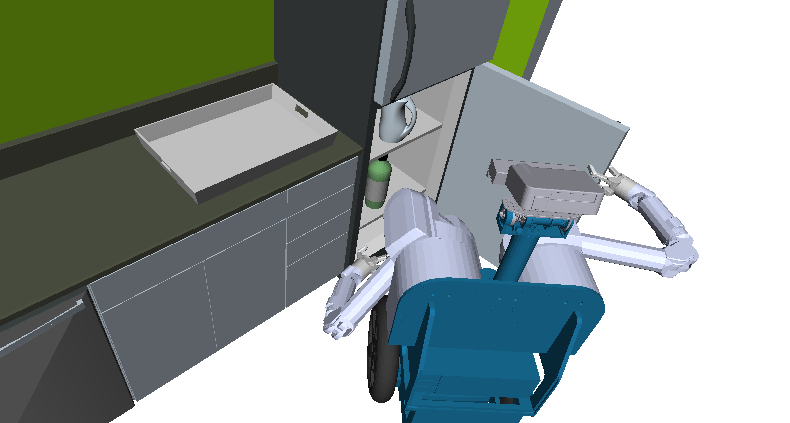
\includegraphics[width=5cm]{figs/fridge-intro.png}};
   
      \node[inner sep=0] at (9,5) {%
         {\only<1>{\includegraphics{build/talk-act1-2d,rootsonly}}}%
         {\only<2>{\includegraphics{build/talk-act1-2d,cfree}}}%
         %{\only<3>{\includegraphics{build/talk-act1-2d,paths}}}%
      };
      
      % legend
      \node[draw,circle,inner sep=2pt,ultra thick,fill=red!50] at (7.05, 2.0) {};
      \node[draw,circle,inner sep=2pt,ultra thick,fill=green!50] at (7.5, 2.0) {};
      \node[anchor=west] at (7.9,2.0) {start, goal configs};
      \only<2->{
         \node[anchor=west,draw,line width=1pt,fill=blue!20,minimum width=0.75cm,minimum height=0.10cm]
            (Cfreebox) at (6.9, 1.5) {};
         \node[anchor=west] at (7.9,1.5) {$\mathcal{C}_{\mbox{\scriptsize free}}$};
      }
      
      %\only<1>{\node at (6,1) {High-dimensional C-space (cite TLP).};}
      %\only<2>{\node at (6,1.3) {\begin{minipage}{11cm}\begin{center}
      %   \begin{equation*}
      %      f_x(\pi) = x(\pi)
      %   \end{equation*}
      %   Lots of possible paths.
      %
      %   {\bf How to find low-cost paths quickly?}%
      %   \end{center}\end{minipage}
      %};}
   
   \end{tikzpicture}
\end{frame}

\begin{frame}
   \frametitle{Motion Planning as Best-First Search over Paths}
   \begin{tikzpicture}
   
      \draw[step=1,black!15,very thin,opacity=\gridopacity] (0,0) grid (12,8);
      
      \node[inner sep=0] at (9,5) {%
         {\only<1>{\includegraphics{build/talk-act1-2d,cfree}}}%
         {\only<2>{\includegraphics{build/talk-act1-2d,paths}}}%
         {\only<3>{\includegraphics{build/talk-act1-2d,traja}}}%
         {\only<4>{\includegraphics{build/talk-act1-2d,firstfail}}}%
         {\only<5>{\includegraphics{build/talk-act1-2d,firstfailnext}}}%
      };
      
      % legend
      \node[draw,circle,inner sep=2pt,ultra thick,fill=red!50] at (7.05, 2.0) {};
      \node[draw,circle,inner sep=2pt,ultra thick,fill=green!50] at (7.5, 2.0) {};
      \node[anchor=west] at (7.9,2.0) {start, goal configs};
      \node[anchor=west,draw,line width=1pt,fill=blue!20,minimum width=0.75cm,minimum height=0.10cm]
         (Cfreebox) at (6.9, 1.5) {};
      \node[anchor=west] at (7.9,1.5) {$\mathcal{C}_{\mbox{\scriptsize free}}$};
      \only<2->{
         \draw[dashed,thick] (6.9,1.0) -- (7.65,1.0);
         \node[anchor=west] at (7.9,1.0) {candidate paths $\Pi$};
      }
      \only<3->{
         \draw[black!30,line width=7pt,line cap=round] (6.9,0.5) -- (7.65,0.5);
         \node[anchor=west] at (7.9,0.5) {path to evaluate ${\hat \pi}^*$};
      }

      % bfs background
      \node[anchor=north,fill=black!5,rounded corners,inner sep=0.2cm,minimum height=3cm,
      minimum width=5.9cm]
      at (3.2,7.5) {};
      
      % bfs highlights
      \only<2,5>{\fill[green!30] (0.25,5.8) rectangle (6.15,6.35);}
      \only<3,5>{\fill[green!30] (0.25,5.1) rectangle (6.15,5.8);}
      \only<4>{\fill[green!30] (0.25,4.6) rectangle (6.15,5.1);}
      
      % bfs text
      \node[anchor=north,inner sep=0.2cm,minimum height=3cm]
      at (3.2,7.5) {\begin{minipage}{5.5cm}
         Best First Search over paths:
         \algrenewcommand\algorithmicindent{0.0cm}%
         \algrenewcommand\algorithmicloop{\!\!\!\!\textbf{loop}}
         \begin{algorithmic}
         \Loop%
            \State $\Pi \leftarrow \mbox{\textsc{GetCandidatePaths}}()$
            \State ${\hat \pi}^* \leftarrow \argmin\limits_{\pi \in \Pi} f(\pi)$
            \State \textsc{EvalPath}$({\hat \pi}^*)$
         \EndLoop
         \end{algorithmic}
      \end{minipage}};
      
      %\only<2>{\node at (6,1) {Select best candidate path.};}
      %\only<3>{\node at (6,1) {Evaluate.};}
   
   \end{tikzpicture}
\end{frame}

%\begin{frame}
%   \frametitle{Best-First Search over Paths}
%   \begin{tikzpicture}
%   
%      \draw[step=1,black!15,very thin,opacity=\gridopacity] (0,0) grid (12,8);
%      
%      \node[inner sep=0] at (9,5) {%
%         {\only<1>{\includegraphics{build/talk-act1-2d,firstfailnext}}}%
%      };
%      
%      % legend
%      \node[anchor=west,draw,line width=1pt,fill=blue!20,minimum width=0.75cm,minimum height=0.10cm]
%         (Cfreebox) at (6.9, 1.9) {};
%      \node[anchor=west] at (7.9,1.9) {$\mathcal{C}_{\mbox{\scriptsize free}}$}; 
%      \draw[dashed,thick] (6.9,1.3) -- (7.65,1.3);
%      \node[anchor=west] at (7.9,1.3) {candidate paths $\Pi$};
%      
%      % bfs background
%      \node[anchor=north,fill=black!5,rounded corners,inner sep=0.2cm,minimum height=3cm,
%      minimum width=5.9cm]
%      at (3.2,7.5) {};
%      
%      % bfs highlights
%      \only<1>{\fill[green!30] (0.25,5.8) rectangle (6.15,6.35);}
%      %\only<2,4>{\fill[green!30] (0.25,5.1) rectangle (6.15,5.8);}
%      %\only<3>{\fill[green!30] (0.25,4.6) rectangle (6.15,5.1);}
%      
%      % bfs text
%      \node[anchor=north,inner sep=0.2cm,minimum height=3cm]
%      at (3.2,7.5) {\begin{minipage}{5.5cm}
%         Best First Search over paths:
%         \algrenewcommand\algorithmicindent{0.0cm}%
%         \algrenewcommand\algorithmicloop{\!\!\!\!\textbf{loop}}
%         \begin{algorithmic}
%         \Loop%
%            \State $\Pi \leftarrow \mbox{\textsc{GetCandidatePaths}}()$
%            \State ${\hat \pi}^* \leftarrow \argmin\limits_{\pi \in \Pi} f(\pi)$
%            \State \textsc{EvalPath}$({\hat \pi}^*)$
%         \EndLoop
%         \end{algorithmic}
%      \end{minipage}};
%      
%   \end{tikzpicture}
%\end{frame}


\begin{frame}
   \frametitle{Best-First Search over Paths: Roadmaps}
   \begin{tikzpicture}
   
      \draw[step=1,black!15,very thin,opacity=\gridopacity] (0,0) grid (12,8);
      
      \node[inner sep=0] at (9,5) {%
         {\only<1>{\includegraphics{build/talk-act1-2d,firstfailnext}}}%
         %{\only<1>{\includegraphics{build/talk-act1-2d,paths}}}%
         {\only<2>{\includegraphics{build/talk-act1-2d,graph}}}%
         %{\only<2>{\includegraphics{build/talk-act1-2d,graphfirst}}}%
         %{\only<3>{\includegraphics{build/talk-act1-2d,graphfirstevaled}}}%
         %{\only<4>{\includegraphics{build/talk-act1-2d,graphfirstnext}}}%
         %{\only<5>{\includegraphics{build/talk-act1-2d,graph}}}%
         {\only<3>{\includegraphics{build/talk-act1-2d,astara}}}%
      };
      
      % legend
      \node[draw,circle,inner sep=2pt,ultra thick,fill=red!50] at (7.05, 2.0) {};
      \node[draw,circle,inner sep=2pt,ultra thick,fill=green!50] at (7.5, 2.0) {};
      \node[anchor=west] at (7.9,2.0) {start, goal configs};
      \node[anchor=west,draw,line width=1pt,fill=blue!20,minimum width=0.75cm,minimum height=0.10cm]
         (Cfreebox) at (6.9, 1.5) {};
      \node[anchor=west] at (7.9,1.5) {$\mathcal{C}_{\mbox{\scriptsize free}}$};
      \draw[dashed,thick] (6.9,1.0) -- (7.65,1.0);
      \node[anchor=west] at (7.9,1.0) {candidate paths $\Pi$};
      
      % bfs background
      \node[anchor=north,fill=black!5,rounded corners,inner sep=0.2cm,minimum height=3cm,
      minimum width=5.9cm]
      at (3.2,7.5) {};
      
      % bfs highlights
      \only<2>{\fill[green!30] (0.25,5.8) rectangle (6.15,6.35);}
      %\only<2,4>{\fill[green!30] (0.25,5.1) rectangle (6.15,5.8);}
      %\only<3>{\fill[green!30] (0.25,4.6) rectangle (6.15,5.1);}
      
      % bfs text
      \node[anchor=north,inner sep=0.2cm,minimum height=3cm]
      at (3.2,7.5) {\begin{minipage}{5.5cm}
         Best First Search over paths:
         \algrenewcommand\algorithmicindent{0.0cm}%
         \algrenewcommand\algorithmicloop{\!\!\!\!\textbf{loop}}
         \begin{algorithmic}
         \Loop%
            \only<1>{\State $\Pi \leftarrow \mbox{\textsc{GetCandidatePaths}}()$}
            \only<2-3>{\State $\Pi \leftarrow \mbox{\textsc{GetRoadmapPaths}}()$}
            \State ${\hat \pi}^* \leftarrow \argmin\limits_{\pi \in \Pi} f(\pi)$
            \State \textsc{EvalPath}$({\hat \pi}^*)$
         \EndLoop
         \end{algorithmic}
      \end{minipage}};
      
      %\only<1-4>{
      %   \node at (6,1) {E.g. Probabalistic RoadMap, state lattice, etc.};
      %}
      
   \end{tikzpicture}
\end{frame}

\begin{frame}
   \frametitle{RRTs as Best-First Search over Paths}
   \begin{tikzpicture}
   
      \draw[step=1,black!15,very thin,opacity=\gridopacity] (0,0) grid (12,8);
      
      \node[inner sep=0] at (9.4,5) {%
         {\only<1>{\includegraphics{build/talk-act1-2d,firstfailnext}}}%
         {\only<2>{\includegraphics{build/talk-act1-2d,rrtstart}}}%
         {\only<3>{\includegraphics{build/talk-act1-2d,rrtsample}}}%
         {\only<4-5>{\includegraphics{build/talk-act1-2d,rrtcandidates}}}%
         {\only<6->{\includegraphics{build/talk-act1-2d,rrtchosen}}}%
      };
      
      % legend
      \node[draw,circle,inner sep=2pt,ultra thick,fill=red!50] at (7.05, 2.0) {};
      \node[draw,circle,inner sep=2pt,ultra thick,fill=green!50] at (7.5, 2.0) {};
      \node[anchor=west] at (7.9,2.0) {start, goal configs};
      \node[anchor=west,draw,line width=1pt,fill=blue!20,minimum width=0.75cm,minimum height=0.10cm]
         (Cfreebox) at (6.9, 1.5) {};
      \node[anchor=west] at (7.9,1.5) {$\mathcal{C}_{\mbox{\scriptsize free}}$};
      \draw[dashed,thick] (6.9,1.0) -- (7.65,1.0);
      \node[anchor=west] at (7.9,1.0) {candidate paths $\Pi$};
      \only<6->{
         \draw[black!30,line width=7pt,line cap=round] (6.9,0.5) -- (7.65,0.5);
         \node[anchor=west] at (7.9,0.5) {path to evaluate ${\hat \pi}^*$};
      }
      
      % bfs background
      \node[anchor=north,fill=black!5,rounded corners,inner sep=0.2cm,minimum height=3cm,
      minimum width=6.6cm]
      at (3.4,7.5) {};
      
      % bfs highlights
      \only<4>{\fill[green!30] (0.1,5.9) rectangle (6.7,6.35);}
      \only<5->{\fill[green!30] (0.1,5.15) rectangle (6.7,6.0);}
      %\only<3>{\fill[green!30] (0.25,4.6) rectangle (6.15,5.15);}
      
      % bfs text
      \node[anchor=north,inner sep=0.1cm,minimum height=3cm]
      at (3.4,7.5) {\begin{minipage}{6.3cm}\small{
         Best First Search over paths:
         \algrenewcommand\algorithmicindent{0.0cm}%
         \algrenewcommand\algorithmicloop{\!\!\!\!\textbf{loop}}
         \begin{algorithmic}
         \Loop%
            \only<1>{\State $\Pi \leftarrow \mbox{\textsc{GetCandidatePaths}}()$}
            \only<2->{\State $\Pi \leftarrow \mbox{\textsc{GetRRTPaths}}()$}
            \State ${\hat \pi}^* \leftarrow \argmin\limits_{\pi \in \Pi}
               \left[ (1-\lambda) \hat{f}_x(\pi) + \lambda \hat{f}_p(\pi) \right]$
            \State \textsc{EvalPath}$({\hat \pi}^*)$
         \EndLoop
         \end{algorithmic}
      }\end{minipage}};
      
      %\only<2>{\node at (6,1) {Select best candidate path.};}
      %\only<3>{\node at (6,1) {Evaluate.};}
      
      \only<7>{
         \node[anchor=north,fill=blue!20,rounded corners,inner sep=0.2cm,
            minimum width=5.9cm,align=center]
         at (3.4,4)
         {
            \bf RRT-Connect is a\\\bf $\lambda=1$ planner!
         };
      }
   
   \end{tikzpicture}
\end{frame}

\begin{frame}
   \frametitle{Best-First Search over Paths: Trajectory Optimization}
   \begin{center}
      \includegraphics{build/talk-act1-2d,traja}
      
      \begin{minipage}{0.65\textwidth}
      \begin{algorithmic}
      \Loop
         \State $\Pi \leftarrow $ \textsc{GetPaths}$()$
            \Comment \tikz{\node[draw,circle,inner sep=0.7pt]{\scriptsize 1};}
         \State $\pi^* \leftarrow \argmin\limits_{\pi \in \Pi} f(\pi)$
            \Comment \tikz{\node[draw,circle,inner sep=0.7pt]{\scriptsize 2};}
         \State \textsc{EvalPath}$(\pi^*)$
            \Comment \tikz{\node[draw,circle,inner sep=0.7pt]{\scriptsize 3};}
      \EndLoop
      \end{algorithmic}
      \end{minipage}
   \end{center}
\end{frame}

\begin{frame}
   \frametitle{Best-First Search over Paths: Trajectory Optimization}
   \begin{center}
      \includegraphics{build/talk-act1-2d,trajb}
      
      \begin{minipage}{0.8\textwidth}
      \begin{algorithmic}
      \Loop
         \State $\Pi \leftarrow $ \textsc{GetPaths}$()$
            \Comment Local neighborhood
         \State $\pi^* \leftarrow \argmin\limits_{\pi \in \Pi} f(\pi)$
            \Comment \tikz{\node[draw,circle,inner sep=0.7pt]{\scriptsize 2};}
         \State \textsc{EvalPath}$(\pi^*)$
            \Comment \tikz{\node[draw,circle,inner sep=0.7pt]{\scriptsize 3};}
      \EndLoop
      \end{algorithmic}
      \end{minipage}
   \end{center}
\end{frame}

\begin{frame}
   \frametitle{Best-First Search over Paths: Trajectory Optimization}
   \begin{center}
      \includegraphics{build/talk-act1-2d,trajc}
      
      \begin{minipage}{0.8\textwidth}
      \begin{algorithmic}
      \Loop
         \State $\Pi \leftarrow $ \textsc{GetPaths}$()$
            \Comment Local neighborhood
         \State $\pi^* \leftarrow \argmin\limits_{\pi \in \Pi} f(\pi)$
            \Comment $f(\pi):$ fuzzy approx
         \State \textsc{EvalPath}$(\pi^*)$
            \Comment \tikz{\node[draw,circle,inner sep=0.7pt]{\scriptsize 3};}
      \EndLoop
      \end{algorithmic}
      \end{minipage}
   \end{center}
\end{frame}

\begin{frame}
   \frametitle{Best-First Search over Paths: Trajectory Optimization}
   \begin{center}
      \includegraphics{build/talk-act1-2d,trajd}
      
      \begin{minipage}{0.8\textwidth}
      \begin{algorithmic}
      \Loop
         \State $\Pi \leftarrow $ \textsc{GetPaths}$()$
            \Comment Local neighborhood
         \State $\pi^* \leftarrow \argmin\limits_{\pi \in \Pi} f(\pi)$
            \Comment $f(\pi):$ fuzzy approx
         \State \textsc{EvalPath}$(\pi^*)$
            \Comment Re-linearize
      \EndLoop
      \end{algorithmic}
      \end{minipage}
   \end{center}
\end{frame}

\begin{frame}
   \frametitle{Graph Search: Edge Execution Effort Model}
   \begin{tikzpicture}
   
      \draw[step=1,black!15,very thin,opacity=\gridopacity] (0,0) grid (12,8);
      
      \node[draw,line width=1.0pt,fill=blue!20,minimum width=0.75cm,minimum height=0.10cm]
         (Cfreebox) at (8.0, 7.5) {};
      \node[right=0cm of Cfreebox] {: $\mathcal{C}_{\mbox{\scriptsize free}}$}; 
      
      \node[inner sep=0] at (10.75,7) {%
         \includegraphics[width=2cm]{build/talk-act1-2d,graph}
      };
      
      % bfs
      \only<1>{\fill[green!30] (0.5,5.6) rectangle (5.5,6.9);}
      \only<2>{\fill[green!30] (0.5,5.6) rectangle (5.5,6.15);}
      \only<3>{\fill[green!30] (0.5,6.15) rectangle (5.5,6.9);}
      \node at (2.5,6.75) {\begin{minipage}{5cm}
         \begin{algorithmic}
         \Loop%
            \State $\Pi \leftarrow $ \textsc{GetPaths}$()$
            \State $\pi^* \leftarrow \argmin\limits_{\pi \in \Pi} f(\pi)$
            \State \textsc{EvalPath}$(\pi^*)$
         \EndLoop
         \end{algorithmic}
         \end{minipage}
      };
      
      \only<2>{
         \fill[green!30] (0.1,3.9) rectangle (5.9,4.9);
         \fill[green!30] (6.1,2.5) rectangle (11.9,4.9);
      }
      \only<3>{
         \fill[green!30] (0.1,2.8) rectangle (5.9,3.9);
         \fill[green!30] (6.1,1.6) rectangle (11.9,2.5);
      }
      
      \node[inner sep=0pt,anchor=north] at (3,5.5) {
         \begin{minipage}[t]{5.5cm}%
            \hrule
            \vspace{0.1cm}
            Distance Model $\mathcal{M}_{\ms{dist}}$
            \begin{algorithmic}[1]
            %\only<2-3>{
               \Function {$x_{\ms{\textup{dist}}}$}{$e$}
                  \State \Return $|| q_e(1) - q_e(0) ||$
               \EndFunction
            %}
            \only<3>{
               \Function {$\hat{x}_{\ms{\textup{dist}}}$}{$e$}
                  \State \Return $|| q_e(1) - q_e(0) ||$
               \EndFunction
            }
            \end{algorithmic}
            \hrule
         \end{minipage}%
      };
      
      \node[inner sep=0pt,anchor=north] at (9,5.5) {
         \begin{minipage}[t]{5.5cm}%
            \hrule
            \vspace{0.1cm}
            Set Validity Model $\mathcal{M}_{\ms{valid}}$
            \only<2-3>{
            \begin{algorithmic}[1]
               \Function {$x_{\ms{\textup{valid}}}$}{$e, \mathcal{C}_{\ms{free}}$}
                  \If {${\bf 1}_{\ms{free}}[q_e(t)]$}
                     \State \Return $0$
                  \Else
                     \State \Return $\infty$
                  \EndIf
               \EndFunction
            \only<3>{
               \Function {$\hat{x}_{\ms{\textup{valid}}}$}{$e, \mathcal{C}_{\ms{free}}$}
                  \State \Return $0$
               \EndFunction
            }
            \end{algorithmic}
            }
            \hrule
         \end{minipage}%
      };
      
      \node at (6,0.5) {
         \begin{minipage}[t]{11cm}
         \centering%
         \only<1>{What is the effort model?}%
         \only<2>{Edge evaluation functions (returns execution effort)}%
         \only<3>{Optimistic (admissible) estimates of execution effort}%
         \only<4>{%
         \vspace{-0.4cm}
         \begin{equation*}
            \hat{f}_x(\pi) = \sum_{e \in \pi} \left\{
            \begin{array}{cl}
               x[e] & \mbox{if edge } e \mbox{ evaluated}  \\
               \hat{x}(e) & \mbox{otherwise} \\
            \end{array}
            \right.
         \end{equation*}
         }%
         \end{minipage}
      };
      
   \end{tikzpicture}
\end{frame}

\begin{frame}
   \frametitle{Why Not Just Run A* Graph Search?}
   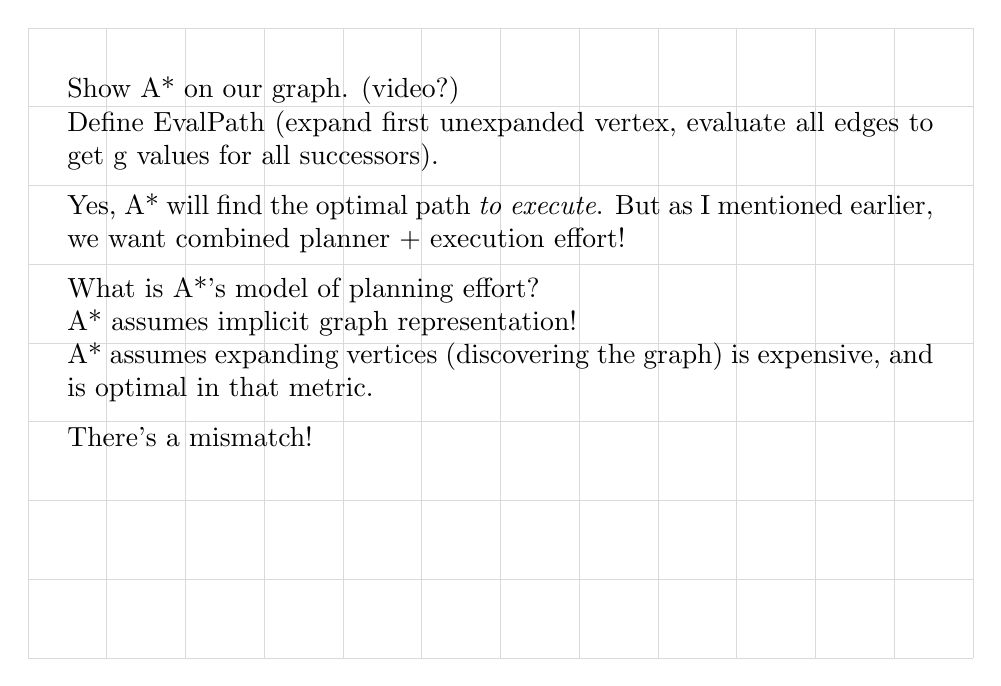
\begin{tikzpicture}
   
      \draw[step=1,black!15,very thin,opacity=\gridopacity] (0,0) grid (12,8);
      
      \node[anchor=north] at (6,7.5)
      {
         \begin{minipage}[t]{11cm}
            Show A* on our graph. (video?)
            
            Define EvalPath (expand first unexpanded vertex,
            evaluate all edges to get g values for all successors).
            
            \medskip
            Yes, A* will find the optimal path \emph{to execute}.
            But as I mentioned earlier, we want combined planner + execution effort!
            
            \medskip
            What is A*'s model of planning effort?
            
            A* assumes implicit graph representation!
            
            A* assumes expanding vertices (discovering the graph)
            is expensive, and is optimal in that metric.
            
            \medskip
            There's a mismatch!
            
         \end{minipage}
      };
      
   \end{tikzpicture}
\end{frame}

\begin{frame}
   \frametitle{Explicit Graph Representation}
   
   Our graphs are small!
   
   Our EvalPath function can be different (e.g. bidirectional).
   Taken from RRTConnect.
   
   Maybe it will perform better?
   
   \begin{equation*}
      \hat{f}_x(\pi) = \sum_{e \in \pi} \left\{
      \begin{array}{cl}
         x[e] & \mbox{if edge } e \mbox{ evaluated}  \\
         \hat{x}(e) & \mbox{otherwise} \\
      \end{array}
      \right.
   \end{equation*}
   
   Similarity to front-to-front algorithms.
   
   This is how Lazy PRM works.
\end{frame}

\begin{frame}
   \frametitle{Roadmaps $\rightarrow$ Graphs}
   \begin{tikzpicture}
   
      \draw[step=1,black!15,very thin,opacity=\gridopacity] (0,0) grid (12,8);
      
      \node[inner sep=0] at (9,5) {%
         {\only<1-4>{\includegraphics{build/talk-act1-2d,graph}}}%
      };
      
      % legend
      \node[draw,line width=1.5pt,fill=blue!20,minimum width=0.75cm,minimum height=0.10cm]
         (Cfreebox) at (3.0, 7.0) {};
      \node[right=0cm of Cfreebox] {: $\mathcal{C}_{\mbox{\scriptsize free}}$}; 
      \node at (3,6.25) {$\Pi$ : set of candidate paths};
      
      \only<1-2>{\fill[green!30] (0.5,3.4) rectangle (5.5,4.1);}
      \only<3>{\fill[green!30] (0.5,2.9) rectangle (5.5,3.4);}
      \only<4>{\fill[green!30] (0.5,3.4) rectangle (5.5,4.1);}
      
      % bfs
      \node at (3,4) {\begin{minipage}{5cm}
         \begin{algorithmic}
         \Loop%
            \State $\Pi \leftarrow $ \textsc{GetPaths}$()$
            \State $\pi^* \leftarrow \argmin\limits_{\pi \in \Pi} f(\pi)$
            \State \textsc{EvalPath}$(\pi^*)$
         \EndLoop
         \end{algorithmic}
         \end{minipage}
      };
      
      \only<2-4>{%
         \node at (6,1) {\begin{minipage}{5cm}%
            \begin{equation*}%
            f(\pi) = {\hat f}_x(\pi) :
            \left\{ \begin{array}{ll}
                x(\pi) & \mbox{if } {\bf 1}_{\mbox{\scriptsize free}}(\pi) \\
                \infty & \mbox{otherwise}
            \end{array} \right.
         \end{equation*}
         \end{minipage}
         };
      }
      
   \end{tikzpicture}
\end{frame}





\begin{frame}
   \frametitle{Best-First Search over Paths: Graphs}
   \begin{center}
      \includegraphics{build/talk-act1-2d,graphfirstnext}
      
      \begin{minipage}{0.65\textwidth}
      \begin{algorithmic}
      \Loop
         \State $\Pi \leftarrow $ \textsc{GetPaths}$()$
            \Comment \tikz{\node[draw,circle,inner sep=0.7pt]{\scriptsize 1};}
         \State $\pi^* \leftarrow \argmin\limits_{\pi \in \Pi} f(\pi)$
            \Comment \tikz{\node[draw,circle,inner sep=0.7pt]{\scriptsize 2};}
         \State \textsc{EvalPath}$(\pi^*)$
            \Comment \tikz{\node[draw,circle,inner sep=0.7pt]{\scriptsize 3};}
      \EndLoop
      \end{algorithmic}
      \end{minipage}
      
      \begin{equation*}
         f_x(\pi) =
         \left\{ \begin{array}{ll}
             x(\pi) & \mbox{if } {\bf 1}_{\mbox{\scriptsize free}}(\pi) \\
             \infty & \mbox{otherwise}
         \end{array} \right.
      \end{equation*}
      
   \end{center}
\end{frame}





\begin{frame}
   \frametitle{Graph Search: Run A*!}
   \begin{tikzpicture}
      \tikzset{>=latex} % arrow heads
   
      \draw[step=1,black!15,very thin,opacity=\gridopacity] (0,0) grid (12,8);
      
      \node[inner sep=0] at (9,5) {%
         {\only<1>{\includegraphics{build/talk-act1-2d,graph}}}%
         {\only<2>{\includegraphics{build/talk-act1-2d,astara}}}%
         {\only<3>{\includegraphics{build/talk-act1-2d,astarb}}}%
         {\only<4>{\includegraphics{build/talk-act1-2d,astarc}}}%
         {\only<5>{\includegraphics{build/talk-act1-2d,astard}}}%
         {\only<6>{\includegraphics{build/talk-act1-2d,astare}}}%
         {\only<7>{\includegraphics{build/talk-act1-2d,astarf}}}%
         {\only<8>{\includegraphics{build/talk-act1-2d,astarg}}}%
         {\only<9>{\includegraphics{build/talk-act1-2d,astarh}}}%
         {\only<10>{\includegraphics{build/talk-act1-2d,astari}}}%
         {\only<11>{\includegraphics{build/talk-act1-2d,astarj}}}%
         {\only<12>{\includegraphics{build/talk-act1-2d,astark}}}%
         {\only<13>{\includegraphics{build/talk-act1-2d,astarl}}}%
         {\only<14>{\includegraphics{build/talk-act1-2d,astarm}}}%
         {\only<15>{\includegraphics{build/talk-act1-2d,astarn}}}%
         {\only<16>{\includegraphics{build/talk-act1-2d,astaro}}}%
         {\only<17>{\includegraphics{build/talk-act1-2d,astarp}}}%
         {\only<18>{\includegraphics{build/talk-act1-2d,astarq}}}%
         {\only<19>{\includegraphics{build/talk-act1-2d,astarr}}}%
         {\only<20-27>{\includegraphics{build/talk-act1-2d,astars}}}%
      };
      
      \node at (3,5.5) {\begin{minipage}{5cm}
         Execution Effort Model:
         \begin{equation*}
            x(e) = \left\{
            \begin{array}{cl}
               ||e|| & \mbox{if } {\bf 1}_{\ms{free}}(e) \\
               \infty & \mbox{otherwise} \\
            \end{array}
            \right.
         \end{equation*}
         Heuristic:
         \begin{equation*}
            {\hat x}(v_a, v_b) = ||v_a - v_b||
         \end{equation*}
         \end{minipage}
      };
      
      \only<21-27>{
         \node at (3,2.25) {Planning Effort Allocation:};
         \draw[] (1,1.5) rectangle (11,2);
      }
      \only<22-27>{
         \draw[fill=yellow] (1.1,1.5) rectangle (1.45,2);
         \node[align=center,inner sep=0] at (0.9,0.8) {\small computing};
         \node[align=center,inner sep=0] at (0.9,0.51) {\small vertex};
         \node[align=center,inner sep=0] at (0.9,0.2) {\small successors};
         \draw[->] (1,1) -- (1.25,1.45);
      }
      \only<23-27>{
         \draw[fill=blue] (1.55,1.5) rectangle (1.95,2);
         \node[align=center,inner sep=0] at (2.8,0.8) {\small sorting};
         \node[align=center,inner sep=0] at (2.8,0.48) {\small open};
         \node[align=center,inner sep=0] at (2.8,0.2) {\small list};
         \draw[->] (2.6,1) -- (1.95,1.45);
      }
      \only<24-27>{
         \draw[fill=red] (2.05,1.5) rectangle (10.9,2);
         \node[align=center,inner sep=0] at (6,0.65) {\small edge};
         \node[align=center,inner sep=0] at (6,0.35) {\small evaluations};
         \draw[->] (6,1) -- (6,1.45);
      }
      
      \only<25-27>{
         \draw[line width=2pt] (1.275,1.75) circle (0.5cm);
      }
      
      \only<26-27>{\node[align=center,fill=white,opacity=0.95] at (7.3,2.9)
         {{\footnotesize Weighted A*}\\{\scriptsize (Pohl 1970)}};}
      \only<27>{\node[align=center,fill=white,opacity=0.95] at (10.2,2.9)
         {{\footnotesize Partial Expansion A*}\\{\scriptsize(Yoshizumi etal. 2000)}};}
      
   \end{tikzpicture}
\end{frame}

\begin{frame}
   \frametitle{Graph Search Mismatch}
   \begin{tikzpicture}
   
      \draw[step=1,black!15,very thin,opacity=\gridopacity] (0,0) grid (12,8);
      
      \node[inner sep=0pt] at (6,7) {\begin{minipage}{12cm}\centering
         A* efficiently addresses {\bf large graphs}, usually represented {\bf implicitly}
         (with {\bf inexpensive edge costs}), by expanding the {\bf fewest vertices}.
      \end{minipage}};
   
      \only<2-4>
      {
         \node[inner sep=0pt] at (2,4.5) {\includegraphics[width=1in]{figs/rubik.png}};
         \node[inner sep=0pt,anchor=north] at (2,2.5)
         {\begin{minipage}{4cm}\centering
            $4.3 \times 10^{19}$ vertices
            
            \tiny{from user Booyabazooka, Wikipedia}
         \end{minipage}};
      }
      
      \only<3-4>
      {
         \node[inner sep=0pt] at (6,4.5) {\includegraphics[width=1in]{figs/15puzzle.png}};
         \node[inner sep=0pt,anchor=north] at (6,2.5)
         {\begin{minipage}{4cm}\centering
            $2.1 \times 10^{13}$ vertices
         \end{minipage}};
      }
      
      \only<4>
      {
         \node[inner sep=0pt] at (10,4.5) {\includegraphics[width=1in]{figs/goldberg-northwest.png}};
         \node[inner sep=0pt,anchor=north] at (10,2.5)
         {\begin{minipage}{4cm}\centering
         
            1.6M vertices
            
            \tiny{
            Goldberg, Harrelson, Kaplan, Werneck.
            ``Efficient Point-to-Point Shortest Path Algorithms''
            }
         \end{minipage}};
      }
   \end{tikzpicture}
\end{frame}

\begin{frame}
   \frametitle{Graph Search Mismatch}
   \begin{tikzpicture}
   
      \draw[step=1,black!15,very thin,opacity=\gridopacity] (0,0) grid (12,8);
      
      \node[inner sep=0pt] at (6,7) {\begin{minipage}{12cm}\centering
         A* efficiently addresses {\bf large graphs}, usually represented {\bf implicitly}
         (with {\bf inexpensive edge costs}), by expanding the {\bf fewest vertices}.
      \end{minipage}};
      
      \only<2-3>{
         \node[inner sep=0pt] at (3.5,4.5) {\includegraphics[width=4cm]{figs/fridge-intro.png}};
         \node[inner sep=0pt,anchor=north] at (3.5,3)
         {\begin{minipage}{4cm}\centering
            Our problem:
         
            $\sim10$k vertices
         \end{minipage}};
      }
      
      \only<3>{
         \node[inner sep=0pt] at (8.5,4.5) {\includegraphics[width=4cm]{figs/prm.png}};
         \node[inner sep=0pt,anchor=north] at (8.5,3)
         {\begin{minipage}{4cm}\centering
            Probabalistic RoadMap
            
            \tiny{Kavraki, Svestka, Latombe, Overmars, 1996}
            
         \end{minipage}};
      }
      
      \only<2-3>{
         \node[inner sep=0pt] at (6,1) {\begin{minipage}{12cm}\centering
            We can represent our graphs {\bf explicitly};
            
            {\bf evaluating graph edges} is expensive,
            
            whereas entire {\bf graph search queries} are inexpensive.
         \end{minipage}};
      }
   
   \end{tikzpicture}
\end{frame}

\begin{frame}
   \frametitle{Roadmaps: Accounting for Spatial Coherence in $\mathcal{C}_{\ms{free}}$}
   \begin{tikzpicture}
   
      \draw[step=1,black!15,very thin,opacity=\gridopacity] (0,0) grid (12,8);
      
      \node[inner sep=0] at (9.4,5) {
         \includegraphics{build/talk-act1-2d,graphfirstevaled}
      };
      
      \node[anchor=north,fill=black!5,rounded corners]
      at (3.4,7.5) {\begin{minipage}{6.3cm}\small{
         Best First Search over paths:
         \algrenewcommand\algorithmicindent{0.0cm}%
         \algrenewcommand\algorithmicloop{\!\!\!\!\textbf{loop}}
         \begin{algorithmic}
         \Loop%
            \State $\Pi \leftarrow \mbox{\textsc{GetRoadmapPaths}}()$
            \State ${\hat \pi}^* \leftarrow \argmin\limits_{\pi \in \Pi}
               \left[ (1-\lambda) \hat{f}_x(\pi) + \lambda \hat{f}_p(\pi) \right]$
            \State \textsc{EvalPath}$({\hat \pi}^*)$
         \EndLoop
         \end{algorithmic}
      }\end{minipage}};
      
      \only<2->{
         \node[anchor=north,fill=blue!20,rounded corners]
         at (3.4,4.7) {\begin{minipage}{6.3cm}\small{
            \begin{itemize}
            \item Roadmap: maintain sparsity
            \item BFS: be optimistic
            \item Densify roadmap on failure
            \end{itemize}
         }\end{minipage}};
      }
      
      \only<3->{
         \node[anchor=north,inner sep=0.3cm,fill=blue!20,rounded corners]
         at (6,2.2) {\begin{minipage}{10cm}\small{\centering
            {\bf What if we optimized ensemble effort \emph{in expectation}?}
            \begin{equation*}
               {\hat \pi}^* \leftarrow \argmin\limits_{\pi \in \Pi}
                  \mbox{E} \left[ (1-\lambda) \hat{f}_x(\pi) + \lambda \hat{f}_p(\pi) \right]
            \end{equation*}
         }\end{minipage}};
      }
      
   \end{tikzpicture}
\end{frame}

\begin{frame}
   \frametitle{Alternative: Optimization in Expectation}
   \begin{tikzpicture}
      \draw[step=1,black!15,very thin,opacity=\gridopacity] (0,0) grid (12,8);
      
      \node[inner sep=0pt] at (6,6)
         {\includegraphics{build/example-in-expectation}};
      
      \only<2->{
         \node[anchor=north,fill=blue!20,rounded corners] at (6,4) {\begin{minipage}{10cm}
            {\bf Research Question Q5:}\\
            Is there a sufficiently expressive and efficient probabilistic
            model of $\mbox{P}_{\ms{free}}(q)$ to allow for minimization
            of ensemble effort in expectation at each iteration?
            
            \medskip
            Starting point: Gaussian Processes for binary classification.
         \end{minipage}};
      }
      
   \end{tikzpicture}
\end{frame}

\begin{frame}
   \frametitle{Efficiency in Graph Search}
   \begin{tikzpicture}
   
      \draw[step=1,black!15,very thin,opacity=\gridopacity] (0,0) grid (12,8);
      
      % example (FIRST) problems
      \only<4-14>
      {
         \node[inner sep=0pt] at (6.5,7) {\includegraphics[width=1.5cm]{figs/rubik.png}};
         \node[inner sep=0pt,anchor=north,align=center,font=\scriptsize] at (6.5,6) {$4.3 \times 10^{19}$\\vertices};
      }
      
      \only<5-14>
      {
         \node[inner sep=0pt] at (8.5,7) {\includegraphics[width=1.5cm]{figs/15puzzle.png}};
         \node[inner sep=0pt,anchor=north,align=center,font=\scriptsize] at (8.5,6) {$2.1 \times 10^{13}$\\vertices};
      }
      
      \only<6-14>
      {
         \node[inner sep=0pt] at (10.5,7) {\includegraphics[width=1.5cm]{figs/goldberg-northwest.png}};
         \node[inner sep=0pt,anchor=north,align=center,font=\scriptsize] at (10.5,6) {1.6M\\vertices};
      }
      
      % example problems SECOND
      \only<17->
      {
         \node[inner sep=0pt] at (2.0,7) {\includegraphics[width=2.5cm]{figs/fridge-intro.png}};
         \node[inner sep=0pt,anchor=north,align=center,font=\scriptsize] at (2.0,6) {$\sim10$k\\vertices};
      }
      \only<18->
      {
         \node[inner sep=0pt] at (5.0,7) {\includegraphics[width=2.5cm]{figs/prm.png}};
         \node[inner sep=0pt,anchor=north,align=center,font=\scriptsize] at (5.0,6)
            {Motivation: PRM};
         % cite
         %\node[anchor=east,font=\scriptsize] at (12,0.5)
         %   {$^\dag$ Kavraki, Svestka, Latombe, Overmars, 1996.};
      }
      
      % draw graph box
      \only<1-2>{
         \node[draw,align=center,minimum height=1.3cm,anchor=south east] at (5,3.5) {
            Graph\\$G = (V,E)$\\\includegraphics[width=1cm]{build/roadmap-2d-simple}
         };
      }
      \only<3-15>{
         \node[draw,align=center,minimum height=1.3cm,anchor=south east] at (5,3.5) {
            Graph\\$G = (V,E)$\\\includegraphics[width=3cm]{build/roadmap-2d-simple}
         };
      }
      % grow using a*!
      \only<7-14>{
         \fill[white,fill opacity=0.9] (1.8,3.6) rectangle (4.9,6.7);
         \begin{scope}
            \clip (1.8,3.6) rectangle (4.9,6.7);
            \only<7>{\clip[rotate around={15:(2.0,4.8)}] (2.0,4.8) ellipse (0.5cm and 0.25cm);}
            \only<8>{\clip[rotate around={15:(2.0,4.8)}] (2.0,4.8) ellipse (1.0cm and 0.50cm);}
            \only<9>{\clip[rotate around={15:(2.0,4.8)}] (2.0,4.8) ellipse (1.4cm and 0.70cm);}
            \only<10>{\clip[rotate around={15:(2.0,4.8)}] (2.0,4.8) ellipse (1.6cm and 0.80cm);}
            \only<11>{\clip[rotate around={15:(2.0,4.8)}] (2.0,4.8) ellipse (1.9cm and 0.85cm);}
            \only<12>{\clip[rotate around={15:(2.0,4.8)}] (2.0,4.8) ellipse (2.1cm and 1.05cm);}
            \only<13-14>{\clip[rotate around={15:(2.0,4.8)}] (2.0,4.8) ellipse (2.2cm and 1.10cm);}
            \node[align=center,minimum height=1.3cm,anchor=south east] at (5,3.5) {
               \includegraphics[width=3cm]{build/roadmap-2d-simple}};
            \only<14>{\draw[rotate around={15:(2.0,4.8)},line width=4pt]
               (2.0,4.8) ellipse (2.2cm and 1.10cm);}
         \end{scope}
      }
      \only<16->{
         \node[draw,align=center,minimum height=1.3cm,anchor=south east,font=\scriptsize] at (5,3.5) {
            Graph\\$G = (V,E)$\\\includegraphics[width=0.5cm]{build/roadmap-2d-simple}
         };
      }
      
      % draw edge eval box
      \only<1-2>{
         \node[draw,align=center,anchor=south west] at (7,3.5)
            {\\Edge Weight\\$x : E \rightarrow \mathbb{R}^+$\\};
      }
      \only<3-15>{
         \begin{scope}[font=\tiny]
            \node[draw,align=center,anchor=south west] at (7,3.5)
               {\\Edge Weight\\$x : E \rightarrow \mathbb{R}^+$\\};
         \end{scope}
      }
      \only<16->{
         \node[draw,align=center,anchor=south west,inner sep=1cm] at (7,3.5)
            {\\Edge Weight\\$x : E \rightarrow \mathbb{R}^+$\\};
      }
      
      \draw[->,line width=1pt] (4,3.25) -- (4,2.75);
      \draw[->,line width=1pt] (8,3.25) -- (8,2.75);
      \node[draw,align=center,minimum height=1.0cm,minimum width=5cm,anchor=north]
         at (6,2.5) {\\$GS(G,x)$};

      % clocks
      \only<2-13>{
         % graph
         \node[fill=white,circle,inner sep=-2pt] at (5,3.5) {\LARGE%
            \only<2-6>{\showclock{0}{0}}%
            \only< 7>{\showclock{0}{10}}%
            \only< 8>{\showclock{0}{20}}%
            \only< 9>{\showclock{0}{30}}%
            \only<10>{\showclock{0}{40}}%
            \only<11>{\showclock{0}{50}}%
            \only<12>{\showclock{1}{00}}%
            \only<13>{\showclock{1}{10}}%
         };
         % edge weight
         \node[fill=white,circle,inner sep=-2pt] at (7,3.5) {\LARGE%
            \only<2-6>{\showclock{0}{0}}%
            \only< 7>{\showclock{0}{5}}%
            \only< 8>{\showclock{0}{10}}%
            \only< 9>{\showclock{0}{15}}%
            \only<10>{\showclock{0}{20}}%
            \only<11>{\showclock{0}{25}}%
            \only<12>{\showclock{0}{30}}%
            \only<13>{\showclock{0}{35}}%
         };
         % graph search
         \node[fill=white,circle,inner sep=-2pt] at (6,2.5) {\LARGE%
            \only<2-6>{\showclock{0}{0}}%
            \only< 7>{\showclock{0}{5}}%
            \only< 8>{\showclock{0}{10}}%
            \only< 9>{\showclock{0}{20}}%
            \only<10>{\showclock{0}{40}}%
            \only<11>{\showclock{1}{20}}%
            \only<12>{\showclock{2}{40}}%
            \only<13>{\showclock{5}{20}}%
         };
      }
      \only<14>{
         % graph
         \node[fill=green,circle,inner sep=-2pt] at (5,3.5) {\LARGE\showclock{1}{10}};
         % edge weight
         \node[fill=white,circle,inner sep=-2pt] at (7,3.5) {\LARGE\showclock{0}{35}};
         % graph search
         \node[fill=white,circle,inner sep=-2pt] at (6,2.5) {\LARGE\showclock{5}{20}};
      }
      \only<15-18>{
         % graph
         \node[fill=white,circle,inner sep=-2pt] at (5,3.5) {\LARGE\showclock{0}{0}};
         % edge weight
         \node[fill=white,circle,inner sep=-2pt] at (7,3.5) {\LARGE\showclock{0}{0}};
         % graph search
         \node[fill=white,circle,inner sep=-2pt] at (6,2.5) {\LARGE\showclock{0}{0}};
      }
      \only<19->{
         % graph
         \node[fill=white,circle,inner sep=-2pt] at (5,3.5) {\LARGE\showclock{0}{0}};
         % edge weight
         \node[fill=green,circle,inner sep=-2pt] at (7,3.5) {\LARGE\showclock{0}{0}};
         % graph search
         \node[fill=white,circle,inner sep=-2pt] at (6,2.5) {\LARGE\showclock{0}{0}};
      }
      
      \node[draw,align=center,shape=document] at (1.5,2) {Query\;\;\;};
      \draw[->,line width=1pt] (2.5,2) -- (3.25,2);
      \draw[->,line width=1pt] (8.75,2) -- (9.50,2);
      \node[draw,align=center,shape=document] at (10.15,2) {$\pi^*$\;\;\;};

      \only<14>{
         \node at (6,0.75) {A* is {\bf optimally efficient} w.r.t
            the number of {\bf vertices considered}.};
      }
      \only<19>{
         \node at (6,0.75) {A* is {\bf not optimally efficient} w.r.t
            the number of {\bf edges evaluated}.
         };
      }
      \only<20>{
         \node[align=center] at (6,0.75) {
            The {\bf E$^4$} graph search problem:\\
            \emph{Explicit graphs with Expensive Edge Evaluations}
         };
      }
      
   \end{tikzpicture}
\end{frame}

\begin{frame}
   \frametitle{Multiple Queries: Relationship to Experience Graphs}
   \begin{tikzpicture}
      \draw[step=1,black!15,very thin,opacity=\gridopacity] (0,0) grid (12,8);
      
      \draw[line width=1pt] (0.5,7.5) -- (11.5,7.5);
      
      \node[align=center] at (3,6.95) {Experience Graphs};
      \node[align=center] at (9,7) {E$^8$ Search};
      
      \draw[line width=0.1pt] (0.5,6.5) -- (11.5,6.5);
      
      \only<2->{
         \node[fill=black!5,rounded corners] at (3,5.75) {\begin{minipage}{4.5cm}\centering\small{
            Only keeping solutions may introduce helpful bias
         }\end{minipage}};
         
         \node[fill=blue!20,rounded corners] at (9,5.75) {\begin{minipage}{4.5cm}\centering\small{
            Keeping all evaluated edges may improve performance
         }\end{minipage}};
      }
      
      \only<3->{
         \node[fill=black!5,rounded corners] at (3,4.5) {\begin{minipage}{4.5cm}\centering\small{
            More efficient for larger graphs (e.g. shortcuts)
         }\end{minipage}};
      }
      
      \only<4->{
         \node[fill=blue!20,rounded corners] at (9,4.5) {\begin{minipage}{4.5cm}\centering\small{
            $\lambda$ and ${\hat{p}}(e)$ may be easier to set than $\epsilon$ and $\epsilon^E$
         }\end{minipage}};
      }
      
      \only<5->{
         \node[fill=blue!20,rounded corners] at (9,3.1) {\begin{minipage}{4.5cm}\centering\small{
            Supports non-proportional planning/execution effort heuristics
         }\end{minipage}};
      }
      
      \only<6->{
         \node[fill=blue!20,rounded corners] at (6,1) {\begin{minipage}{9cm}
            {\bf Research Question Q3:}\\
            How does the explicit graph approach of E$^8$ compare to
            weighted and anytime implicit algorithms?
         \end{minipage}};
      }
      
   \end{tikzpicture}
\end{frame}

\begin{frame}
   \frametitle{Continuous Spaces: Ensemble Effort Models}
   \begin{tikzpicture}
   
      \draw[step=1,black!15,very thin,opacity=\gridopacity] (0,0) grid (12,8);
      
      \node at (3,6.75) {e.g. $\mathcal{M} = \mathcal{M}_{\ms{dist}}
         + \mathcal{M}_{\ms{valid}}(\mathcal{C}_{\ms{free}})$};
      
      \node[inner sep=0] at (8,6.75) {%
         \includegraphics[width=2cm]{build/talk-act1-2d,graph}
      };
      \node[draw,line width=1.0pt,fill=blue!20,minimum width=0.75cm,minimum height=0.10cm]
         (Cfreebox) at (9.75, 6) {};
      \node[right=0cm of Cfreebox] {: $\mathcal{C}_{\ms{free}}$}; 
      
      \node[draw,shape=document,anchor=north] at (3,5.5) {
         \begin{minipage}[t]{5.5cm}%
            \vspace{0.1cm}
            Distance Model $\mathcal{M}_{\ms{dist}}$
            \begin{algorithmic}[1]
            \Function {$x_{\ms{\textup{dist}}}$}{$e$}
               \State \Return $|| q_e(1) - q_e(0) ||$
            \EndFunction
            \Function {$\hat{x}_{\ms{\textup{dist}}}$}{$e$}
               \State \Return $|| q_e(1) - q_e(0) ||$
            \EndFunction
            \Function {$\hat{p}_{\ms{\textup{dist}}}$}{$e$}
               \State \Return $0$
            \EndFunction
            \end{algorithmic}
         \end{minipage}%
      };
      
      \node[draw,shape=document,anchor=north] at (9,5.5) {
         \begin{minipage}[t]{5.5cm}%
            \vspace{0.1cm}
            Set Validity Model $\mathcal{M}_{\ms{valid}}(\mathcal{C}_{\ms{free}})$
            \begin{algorithmic}[1]
            \Function {$x_{\ms{\textup{valid}}}$}{$e, \mathcal{C}_{\ms{free}}$}
               \If {${\bf 1}_{\ms{free}}[q_e(t)]$}
                  \State \Return $0$
               \Else
                  \State \Return $\infty$
               \EndIf
            \EndFunction
            \Function {$\hat{x}_{\ms{\textup{valid}}}$}{$e, \mathcal{C}_{\ms{free}}$}
               \State \Return $0$
            \EndFunction
            \Function {$\hat{p}_{\ms{\textup{valid}}}$}{$e, \mathcal{C}_{\ms{free}}$}
               \State \Return $\hat{p}_{\ms{\textup{free}}}[q_e(t)]$
            \EndFunction
            \end{algorithmic}
         \end{minipage}%
      };
      
   \end{tikzpicture}
\end{frame}

\begin{frame}
   \frametitle{Multi-Set Instances: Conservative Robot Models}
   \begin{tikzpicture}
      \draw[step=1,black!15,very thin,opacity=\gridopacity] (0,0) grid (12,8);
      
      \node[inner sep=0pt] at (2.8,4) {%
         \only<1>{\includegraphics[height=7.5cm]{figs/herb-fridge-sets-j.png}}%
         \only<2-4>{\includegraphics[height=7.5cm]{figs/herb-fridge-sets-k.png}}%
      };
      
      \node[anchor=north,fill=black!15,rounded corners,font=\small]
      at (8.8,7.75) {\begin{minipage}{6cm}
         The valid set $S_R$ while grabbing the object
         can be conservatively bounded by a simpler geometry
         yielding $S_B$.
      \end{minipage}};
      
      \node[inner sep=0pt] at (8.8,4) {%
         \only<1>{\includegraphics[width=4.5cm]{build/multiset-manip-instances-blob,routside}}%
         \only<2>{\includegraphics[width=4.5cm]{build/multiset-manip-instances-blob,rinside}}%
         \only<3>{\includegraphics[width=6cm]{build/broadphase-single}}%
         \only<4>{\includegraphics[width=6cm]{build/broadphase-multi}}%
      };
   
   \end{tikzpicture}
\end{frame}

\begin{frame}
   \frametitle{Multi-Set Validitiy Effort Model}
   \begin{tikzpicture}
      \draw[step=1,black!15,very thin,opacity=\gridopacity] (0,0) grid (12,8);

      \node[draw,shape=document,font=\scriptsize] at (6,4) {
         \begin{minipage}[t]{11cm}%
            \vspace{0.1cm}
            Multi-Set Validitiy Effort Model $\mathcal{M}_{\ms{multi}}$
            \medskip
            {\algrenewcommand\textproc{}% Used to be \textsc
            \begin{algorithmic}[1]
            \Function {$x_{\ms{multi}}$}{$e, S_u$}
               \State $(\mathcal{F}_{\ms{cert}}, b_{\ms{cert}}, {\hat p}_{\ms{cert}})
                  \leftarrow \mbox{\sc MultiOptCert}(q_e, S_u,
                  P_{\ms{global}} \cup e.P_{\ms{eval}})$
               \ForAll {$S \in \mathcal{F}_{\ms{cert}}$}
                  \State $b_{\ms{eval}} \leftarrow \mathbf{1}_S[q_e]$
                  \State $\arraycolsep=2pt
                     e.P_{\ms{eval}} \leftarrow e.P_{\ms{eval}} \cup
                     \left\{\begin{array}{rl}
                     \mathbf{1}_S & \mbox{if } b_{\ms{eval}} \\
                     \lnot \mathbf{1}_S & \mbox{otherwise} \\
                     \end{array}
                     \right\}$
                  \If {$b_{\ms{eval}} \neq b_{\ms{cert}}(S)$}
                     \State \Return $\infty$
                  \EndIf
               \EndFor
               \State \Return $0$
            \EndFunction
            \medskip
            \Function {$\hat{x}_{\ms{multi}}$}{$e, S_u$}
               \State \Return $0$
            \EndFunction
            \medskip
            \Function {$\hat{p}_{\ms{multi}}$}{$e, S_u$}
               \State $(\mathcal{F}_{\ms{cert}}, b_{\ms{cert}}, {\hat p}_{\ms{cert}})
                  \leftarrow \mbox{\sc MultiOptCert}(q_e, S_u,
                  P_{\ms{global}} \cup e.P_{\ms{eval}})$
               \State \Return ${\hat p}_{\ms{cert}}$
            \EndFunction
            \end{algorithmic}
            } %textproc
         \end{minipage}%
      };
   
   \end{tikzpicture}
\end{frame}

\begin{frame}
   \frametitle{CMR as an Edge Queue}
   \begin{tikzpicture}
      \draw[step=1,black!15,very thin,opacity=\gridopacity] (0,0) grid (12,8);
      
      \node[inner sep=0pt] at (6,6.5)
         {\includegraphics{build/cmr-queue-intro}};
      
      \draw[thick] (1.5,5.3) -- (10.5,5.3);
      \node[inner sep=0pt] at (6,4.0)
         {\includegraphics{build/cmr-simpleex-classical}};
      \draw[thin] (1.5,2.7) -- (10.5,2.7);
      \node[inner sep=0pt] at (6,1.4)
         {\includegraphics{build/cmr-simpleex-colored}};
      \draw[thick] (1.5,0.1) -- (10.5,0.1);
   
   \end{tikzpicture}
\end{frame}

\begin{frame}
   \frametitle{CMR Example}
   \begin{tikzpicture}
      \draw[step=1,black!15,very thin,opacity=\gridopacity] (0,0) grid (12,8);
      
      \node[draw] at (6,4)
      {
         \includegraphics{build/w13-fu1-ec86}
      };
   
   \end{tikzpicture}
\end{frame}

\begin{frame}
   \frametitle{Multi-Set Instances: Dynamic Environments}
   \begin{tikzpicture}
      \draw[step=1,black!15,very thin,opacity=\gridopacity] (0,0) grid (12,8);
      
      \node[inner sep=0pt] at (2.8,4) {%
         \only<1>{\includegraphics[height=7.5cm]{figs/herb-fridge-sets-b.png}}%
         \only<2>{\includegraphics[height=7.5cm]{figs/herb-fridge-sets-a.png}}%
         \only<3>{\includegraphics[height=7.5cm]{figs/herb-fridge-sets-b.png}}%
      };
      
      \node[anchor=north,fill=black!15,rounded corners,font=\small]
      at (8.8,7.75) {\begin{minipage}{6cm}
         The valid set $S_A$ in the presence of an object
         is a subset of the valid set $S_N$ with the object removed.
      \end{minipage}};
      
      \node[inner sep=0pt] at (8.8,4) {%
         \only<1>{\includegraphics[width=4.5cm]{build/multiset-manip-instances,dyna}}%
         \only<2>{\includegraphics[width=4.5cm]{build/multiset-manip-instances,dynb}}%
         \only<3>{\includegraphics[width=4.5cm]{build/multiset-manip-instances,dync}}%
      };
      
   \end{tikzpicture}
\end{frame}

\begin{frame}
   \frametitle{Multi-Set Instances: Dynamic Environments}
   \begin{tikzpicture}
      \draw[step=1,black!15,very thin,opacity=\gridopacity] (0,0) grid (12,8);
      
      \begin{scope}[shift={(1,1.2)},font=\small]
         \node[anchor=south west,inner sep=0] at (0,0)
           {\includegraphics[width=5.2cm]{figs/chimp-voxels-delta.png}};

         \node[draw,inner sep=3pt,fill=white,fill opacity=0.9,align=center]
           (debrislab) at (0.7,1.0) {Debris object\\removed};
         \node[circle,inner sep=2,draw,fill=white] (debris) at (2.2,2.9) {};
         \draw[draw=black, double=white, double distance=1pt, line width=1pt]
           (debrislab.north) -- (debris);
           
         \node[draw,inner sep=3pt,fill=white,fill opacity=0.9,align=center]
           (addlab) at (5.0,2.0) {Additional\\voxels seen};
         \node[circle,inner sep=2,draw,fill=white] (added) at (4.4,5.0) {};
         \draw[draw=black, double=white, double distance=1pt, line width=1pt]
           (addlab.north) -- (added);
      \end{scope}
      
      \node[inner sep=0pt] at (9.5,6) {
         \includegraphics{build/retroactive-a}
      };
      
      \node[inner sep=0pt] at (9.5,2) {
         \includegraphics{build/retroactive-b}
      };
   \end{tikzpicture}
\end{frame}

\begin{frame}
   \frametitle{Multi-Set Instances: Grasped Objects}
   \begin{tikzpicture}
      \draw[step=1,black!15,very thin,opacity=\gridopacity] (0,0) grid (12,8);
      
      \node[inner sep=0pt] at (2.8,4) {%
         \only<1>{\includegraphics[height=7.5cm]{figs/herb-fridge-sets-c.png}}%
         \only<2>{\includegraphics[height=7.5cm]{figs/herb-fridge-sets-a.png}}%
         \only<3>{\includegraphics[height=7.5cm]{figs/herb-fridge-sets-c.png}}%
      };
      
      \node[anchor=north,fill=black!15,rounded corners,font=\small]
      at (8.8,7.75) {\begin{minipage}{6cm}
         The valid set $S_A$ while grasping an object
         is a subset of the valid set $S_N$ with the object removed.
      \end{minipage}};
      
      \node[inner sep=0pt] at (8.8,4) {%
         \only<1>{\includegraphics[width=4.5cm]{build/multiset-manip-instances,dyna}}%
         \only<2>{\includegraphics[width=4.5cm]{build/multiset-manip-instances,dynb}}%
         \only<3>{\includegraphics[width=4.5cm]{build/multiset-manip-instances,dync}}%
      };
      
   \end{tikzpicture}
\end{frame}

\begin{frame}
   \frametitle{Multi-Set Instances: Self-Collision Checking}
   \begin{tikzpicture}
      \draw[step=1,black!15,very thin,opacity=\gridopacity] (0,0) grid (12,8);

      \node[inner sep=0pt] at (2.8,4) {%
         \only<1>{\includegraphics[height=7.5cm]{figs/herb-fridge-sets-a.png}}%
         \only<2>{\includegraphics[height=7.5cm]{figs/herb-fridge-sets-d.png}}%
         \only<3>{\includegraphics[height=7.5cm]{figs/herb-fridge-sets-a.png}}%
      };

      \node[anchor=north,fill=black!15,rounded corners,font=\small]
      at (8.8,7.75) {\begin{minipage}{6cm}
         The valid set $S_A$
         is a subset of the valid set $S_R$
         consisting of robot self-collision-free configurations.
      \end{minipage}};

      \node[inner sep=0pt] at (8.8,4) {%
         \only<1>{\includegraphics[width=4.5cm]{build/multiset-manip-instances,selfa}}%
         \only<2>{\includegraphics[width=4.5cm]{build/multiset-manip-instances,selfb}}%
         \only<3>{\includegraphics[width=4.5cm]{build/multiset-manip-instances,selfc}}%
      };

   \end{tikzpicture}
\end{frame}

\begin{frame}
   \frametitle{Multi-Set Instances: Conservative Obstacle Volumes}
   \begin{tikzpicture}
      \draw[step=1,black!15,very thin,opacity=\gridopacity] (0,0) grid (12,8);
      
      \node[inner sep=0pt] at (2.8,4) {%
         \only<1>{\includegraphics[height=7.5cm]{figs/herb-fridge-sets-h.png}}%
         \only<2-3>{\includegraphics[height=7.5cm]{figs/herb-fridge-sets-e.png}}%
      };
      
      \node[anchor=north,fill=black!15,rounded corners,font=\small]
      at (8.8,7.75) {\begin{minipage}{6cm}
         The valid set $S_O$ in the presence of an object
         can be conservatively bounded by a simpler geometry
         yielding $S_B$.
      \end{minipage}};
      
      \node[inner sep=0pt] at (8.8,4) {%
         \only<1>{\includegraphics[width=4.5cm]{build/multiset-manip-instances-blob,outside}}%
         \only<2->{\includegraphics[width=4.5cm]{build/multiset-manip-instances-blob,inside}}%
      };
      
      \only<3->{
         \node[anchor=north,fill=black!15,rounded corners,font=\small]
         at (8.8,2) {\begin{minipage}{6cm}
            Extreme case: Leven/Hutchinson workcell decomposition.
         \end{minipage}};
      }
      
   \end{tikzpicture}
\end{frame}

\begin{frame}
   \frametitle{Multi-Set Instances: Conservative Grasped Volumes}
   \begin{tikzpicture}
      \draw[step=1,black!15,very thin,opacity=\gridopacity] (0,0) grid (12,8);
      
      \node[inner sep=0pt] at (2.8,4) {%
         \only<1>{\includegraphics[height=7.5cm]{figs/herb-fridge-sets-c.png}}%
         \only<2>{\includegraphics[height=7.5cm]{figs/herb-fridge-sets-i.png}}%
      };
      
      \node[anchor=north,fill=black!15,rounded corners,font=\small]
      at (8.8,7.75) {\begin{minipage}{6cm}
         The valid set $S_O$ while grabbing the object
         can be conservatively bounded by a simpler geometry
         yielding $S_B$.
      \end{minipage}};
      
      \node[inner sep=0pt] at (8.8,4) {%
         \only<1>{\includegraphics[width=4.5cm]{build/multiset-manip-instances-blob,outside}}%
         \only<2>{\includegraphics[width=4.5cm]{build/multiset-manip-instances-blob,inside}}%
      };

   \end{tikzpicture}
\end{frame}

\begin{frame}
   \frametitle{Multi-Set Instances: Conservative Robot Models}
   \begin{tikzpicture}
      \draw[step=1,black!15,very thin,opacity=\gridopacity] (0,0) grid (12,8);
      
      \node[inner sep=0pt] at (2.8,4) {%
         \only<1>{\includegraphics[height=7.5cm]{figs/herb-fridge-sets-j.png}}%
         \only<2->{\includegraphics[height=7.5cm]{figs/herb-fridge-sets-k.png}}%
      };
      
      \node[anchor=north,fill=black!15,rounded corners,font=\small]
      at (8.8,7.75) {\begin{minipage}{6cm}
         The valid set $S_R$ while grabbing the object
         can be conservatively bounded by a simpler geometry
         yielding $S_B$.
      \end{minipage}};
      
      \node[inner sep=0pt] at (8.8,4) {%
         \only<1>{\includegraphics[width=4.5cm]{build/multiset-manip-instances-blob,routside}}%
         \only<2>{\includegraphics[width=4.5cm]{build/multiset-manip-instances-blob,rinside}}%
      };
   
   \end{tikzpicture}
\end{frame}


